\scanpage{53}
\mspage{6}
L'isom. canonique déduit de l'inclusion.

On a de plus des isomorphismes canoniques
\[
(30)\quad\left\{\begin{aligned}
\varphi_{i\varepsilon}&:\Pi_\omega\longrightarrow\Pi_i\qquad\text{défini par }c_i^\varepsilon:P_\varepsilon\longrightarrow Q_i\\
\varphi_{\varepsilon i}&:\Pi_i\longrightarrow\Pi_\omega\qquad\text{---}\qquad(c_i^\varepsilon)^{-1}:Q_i\longrightarrow P_\varepsilon
\end{aligned}\right.
\]
\margin{\begin{tabular}{@{}l@{}}
\uline{NB} on a\\
$\varphi_{i\varepsilon}=\varphi_{Q_i,\varepsilon}$\\
$\varphi_{\varepsilon i}=\varphi_{P_\varepsilon,i}$
\end{tabular}}
Par ces isom, les $\Pi_{\unsure{\varepsilon}},\Pi_i$ sont reliés de façon transitive, mais bien entendu pas par un syst. transitif d'isomorphismes -- au contraire, les autom d'un des groupes $\Pi_{\unsure{\varepsilon}},\Pi_i$ obtenus en composant des \unsure{isoms|isom} (30) suivant des chemins fermés sur le graphe
\figure{
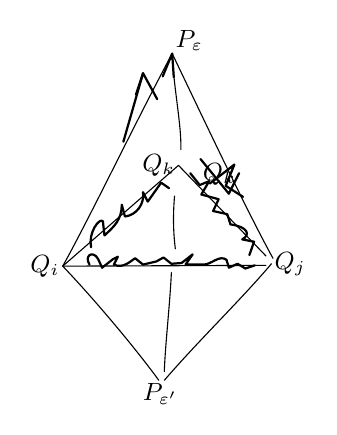
\begin{tikzpicture}[x=1cm,y=1cm,line cap=round,line join=round,every node/.style={font=\small,inner sep=1pt}]
\coordinate (P) at (.02,2.70);
\coordinate (I) at (-1.37,0);
\coordinate (J) at (1.28,.03);
\coordinate (K) at (.10,1.28);
\coordinate (M) at (-.13,-1.45);
\draw (P) .. controls (-.42,1.88) and (-1.02,.63) .. (I);
\draw (P) .. controls (.47,1.76) and (.98,.68) .. (1.30,.10);
\draw (I) .. controls (-.94,-.45) and (-.41,-1.09) .. (-.15,-1.45);
\draw (-.08,-1.45) .. controls (.35,-.95) and (.91,-.41) .. (J);
\draw (P) .. controls (.04,2.25) and (.14,1.79) .. (.13,1.48);
\draw (.05,.89) .. controls (.025,.60) and (.04,.38) .. (.06,.22);
\draw (.01,-.08) .. controls (-.01,-.50) and (-.07,-1.02) .. (-.08,-1.34);
\draw (I)--(K)--(1.21,.13);
\draw (I)--(1.21,.01);
\draw[thick] (-.60,1.58)--(-.35,2.45);
\draw[thick] (-.44,2.18)--(-.35,2.45)--(-.17,2.12);
\draw[thick] (-.10,2.41)--(.02,2.70)--(.04,2.40);
\draw[thick] (-1.01,.24).. controls (-1.05,.43) and (-.90,.62)..(-.86,.57)
  --(-.84,.39).. controls (-.72,.50) and (-.62,.59)..(-.62,.78)
  --(-.58,.63).. controls (-.43,.65) and (-.33,.79)..(-.35,.94)
  --(-.29,.82)--(-.12,1.06)--(-.02,.99);
\draw[thick] (.25,1.18)--(.37,1.03)--(.49,1.08)--(.39,.91)
  --(.61,.85)--(.54,.70)--(.72,.66)--(.76,.53)
  .. controls (.98,.50) and (1.02,.40)..(.91,.34)
  --(1.06,.31)--(1.00,.14);
\draw[thick] (-1.03,.02).. controls (-1.10,.13) and (-.99,.21)..(-.92,.09)
  --(-.87,-.02)--(-.73,.09)--(-.67,.12)--(-.72,.02)
  .. controls (-.60,-.04) and (-.49,.08)..(-.45,.10)
  --(-.35,.02)--(-.18,.06)--(-.09,.11)--(.01,.03)
  --(.14,.04)--(.28,.15)--(.19,.02)--(.42,.02)
  .. controls (.52,.02) and (.62,.15)..(.71,.08)
  --(.74,-.02)--(.85,.03)--(.95,-.03)--(1.07,.01);
\node[above right] at (P) {$P_{\unsure{\varepsilon}}$};
\node[below] at (M) {$P_{\varepsilon'}$};
\node[left] at (I) {$Q_i$};
\node[right] at (J) {$Q_j$};
\node[left] at (K) {$Q_k$};
\node at (.62,1.16) {$\deleted{\unsure{Q_k}}$};
\draw[thick] (.38,1.36)--(.74,.92)--(.87,1.18);
\draw[thick] (.50,1.05)--(.81,1.29)--(.70,1.02)--(.92,.88);
\end{tikzpicture}
}
sont \uline{tous} les autom. intérieurs !

Les $\Pi_1(\unsure{\overline{\Sigma}|\widetilde{\Sigma}}^{*},\text{en }-)$ en les $P_\varepsilon,Q_i$ étant canonifiés comme les $\Pi_\varepsilon,\Pi_i$, il reste \unsure{à|:} ``repérer'' les $\Pi_1$ en les autres sommets marqués jusqu'à maintenant. Les choix naturels sont par
\deleted{$\unsure{\varphi}_{\unsure{\omega|\varepsilon}}\ \Pi_i\quad\unsure{\varphi|\Pi}_{\unsure{\varepsilon}i}\ \Pi_i\longrightarrow$}
\margin{52}
